%% 
%% Copyright 2007, 2008, 2009 Elsevier Ltd
%% 
%% This file is part of the 'Elsarticle Bundle'.
%% ---------------------------------------------
%% 
%% It may be distributed under the conditions of the LaTeX Project Public
%% License, either version 1.2 of this license or (at your option) any
%% later version.  The latest version of this license is in
%%    http://www.latex-project.org/lppl.txt
%% and version 1.2 or later is part of all distributions of LaTeX
%% version 1999/12/01 or later.
%% 
%% The list of all files belonging to the 'Elsarticle Bundle' is
%% given in the file `manifest.txt'.
%% 

%% Template article for Elsevier's document class `elsarticle'
%% with numbered style bibliographic references
%% SP 2008/03/01

\documentclass[12pt,times,twocolumn,3p]{elsarticle}

%% Use the option review to obtain double line spacing
%% \documentclass[authoryear,preprint,review,12pt]{elsarticle}

%% Use the options 1p,twocolumn; 3p; 3p,twocolumn; 5p; or 5p,twocolumn
%% for a journal layout:
%% \documentclass[final,1p,times]{elsarticle}
%% \documentclass[final,1p,times,twocolumn]{elsarticle}
%% \documentclass[final,3p,times]{elsarticle}
%% \documentclass[final,3p,times,twocolumn]{elsarticle}
%% \documentclass[final,5p,times]{elsarticle}
%% \documentclass[final,5p,times,twocolumn]{elsarticle}

%% For including figures, graphicx.sty has been loaded in
%% elsarticle.cls. If you prefer to use the old commands
%% please give \usepackage{epsfig}

%% The amssymb package provides various useful mathematical symbols
\usepackage{amssymb}
%% The amsthm package provides extended theorem environments
%% \usepackage{amsthm}

%% The lineno packages adds line numbers. Start line numbering with
%% \begin{linenumbers}, end it with \end{linenumbers}. Or switch it on
%% for the whole article with \linenumbers.
%% \usepackage{lineno}

%% To generate filler text
\usepackage[english]{babel}
\usepackage{blindtext}

%% Used for making nice references
\usepackage{hyperref}
\usepackage{cleveref}
\usepackage{cuted}
\usepackage{siunitx}

\journal{Materials Science}

\begin{document}

\begin{frontmatter}

%% Title, authors and addresses

%% use the tnoteref command within \title for footnotes;
%% use the tnotetext command for theassociated footnote;
%% use the fnref command within \author or \address for footnotes;
%% use the fntext command for theassociated footnote;
%% use the corref command within \author for corresponding author footnotes;
%% use the cortext command for theassociated footnote;
%% use the ead command for the email address,
%% and the form \ead[url] for the home page:
%% \title{Title\tnoteref{label1}}
%% \tnotetext[label1]{}
%% \author{Name\corref{cor1}\fnref{label2}}
%% \ead{email address}
%% \ead[url]{home page}
%% \fntext[label2]{}
%% \cortext[cor1]{}
%% \address{Address\fnref{label3}}
%% \fntext[label3]{}

\title{Finite Element Analysis of Thin Disk in Fortran}

%% use optional labels to link authors explicitly to addresses:
%% \author[label1,label2]{}
%% \address[label1]{}
%% \address[label2]{}

\author{B.~Himberg}

\address{}

\begin{abstract}
%% Text of abstract
Finite Element Methods are ubiquitous in Materials Science. They represent the
melding of boundary conditions and partial differential equations. Here such a
method combines a fourth order partial differential equation in polar coordinates
with a simply supported circular plate. Focusing on the maximum deflection, a
comparison of of this finite element method is made to the analytic results for
a steel plate under uniform pressure. The primary contribution to error is found
to be the ratio of plate thickness to plate support length, proportional to the
radius here.

\end{abstract}

\begin{keyword}
%% keywords here, in the form: keyword \sep keyword
Finite Element Method \sep Finite Element Analysis \sep Thin Plate

%% PACS codes here, in the form: \PACS code \sep code

%% MSC codes here, in the form: \MSC code \sep code
%% or \MSC[2008] code \sep code (2000 is the default)

\end{keyword}

\end{frontmatter}

%% \linenumbers

%% main text
\section{Introduction} \label{intro}
Typically analytic solutions are limited to simpler conditions, however these
solutions can be used to validate numerical methods. Once benchmarked, such
numerical methods can then be used to evaluate properties of much more complex problems.
This paper presents a comparison of the Finite Element Method to an analytic
solution with a focus on sources of error due to support length ratio and
pressure, material specifics such as Young's Modulus or Poisson's
Ratio, and finally tunable parameters such as the number of finite elements.

The benchmark used here is the maximum deflection of a simply supported circular
thin plate under uniform pressure. Simply supported means that the edges are
fixed: any node on the edge is constrained to remain stationary. Intuition
suggests that the plate will have greater deflection away from the edges,
leading to maximum deflection at the center of the plate.

The analytic solution and finite element method share the same differential
equation, to be found in \cite{zien,boresi}. High level details are presented in
\cref{sec:ana} before the finite element method used here, a Fortran implementation
\cite{geocities} which this author has modified for extended capabilities, is
discussed in \cref{sec:fem}. Graphical results can be found in \cref{sec:comp},
followed by a discussion of future work in \cref{sec:disc}.

Finally note that all the data, and the code used to obtain it, can be found
on GitHub \cite{github} as well as the source code and graphs for this paper.

\section{Analytic Method} \label{sec:ana}
Both the analytic solution and finite element method begin with the same
differential equation
\begin{equation} \label{eqn:dp}
\Delta^2\Delta^2 w = \frac{P}{D}
\end{equation}
where $P$ is the pressure and $D$ is the flexural rigidity. This is the most
general form, and is also a starting point for square plates.


The Laplacian operator is often involved in finite element methods. Here we use
its polar coordinates definition to arrive at

\begin{strip}
\noindent\makebox[\linewidth][l]{\rule{0.4\textwidth}{0.4pt}}
\begin{equation} \label{eqn:dp2}
\Delta^2\Delta^2 w =
\left(\frac{\partial^2}{\partial r^2} +
\frac{1}{r}\frac{\partial}{\partial r} +
\frac{1}{r^2}\frac{\partial^2}{\partial \theta^2}\right)
\left(\frac{\partial^2 w}{\partial r^2} +
\frac{1}{r}\frac{\partial w}{\partial r} +
\frac{1}{r^2}\frac{\partial^2 w}{\partial \theta^2}\right) =
\frac{P}{D}
\end{equation}
\begin{flushleft}
\noindent\makebox[\linewidth][r]{\rule{0.4\textwidth}{0.4pt}}
\end{flushleft}
\end{strip}

\noindent which may be simplified by supporting the plate symmetrically with
respect to the z-axis. This eliminates the $\theta$ dependency of \cref{eqn:dp2},
leading to
\begin{equation} \label{eqn:dp3}
\left(\frac{\partial^2}{\partial r^2} +
\frac{1}{r}\frac{\partial}{\partial r}
\right)
\left(\frac{\partial^2 w}{\partial r^2} +
\frac{1}{r}\frac{\partial w}{\partial r}
\right) = \frac{P}{D}
\end{equation}
for which the solution
\begin{equation}
w(r) = \frac{P r^4}{64 D} +A_1 +B_1 r^2
\end{equation}
exists. The case of simply supported edges can be shown \cite{boresi} to yield
\begin{equation} \label{eqn:df4}
w(r) = \frac{P a^4}{64 D}
\left[1-\left(\frac{r}{a}\right)^2\right]
\left[\frac{5+\nu}{1+\nu}-\left(\frac{r}{a}\right)^2\right]
\end{equation}
which presents the new variables $a$, the radius of the disk, and Poisson's Ratio
$\nu$. Here $r$ is the point at which deflection is measured and, happening to be
the origin, simplifies the equation even further. First though, flexural rigidity
may be defined as
\begin{equation}
D = \frac{E^2 h^3}{12(1 - \nu^2)}
\end{equation}
which is applied to \cref{eqn:df4} to arrive the final expression
\begin{equation} \label{eqn:def}
w_{max}(a) = \frac{3 P a^4}{16 E h^3}(5+v)(1-v)
\end{equation}
for $w_{max}$, the maximum deflection at the center of a disc under uniform
constant pressure $p$. Here $E$ and $\nu$ are Young's Modulus and Poisson's ratio,
properties of the material the disc is comprised of. The height $h$ and radius $r$
are measurements of the spatial extent of the disc, and their ratio must be
i$h/r < 0.1$ in order to match with experimental results \cite{boresi}.

\section{Finite Element Method} \label{sec:fem}
Finite element methods (FEMs) have a very specific set of requirements: boundary
conditions, on an equation describing the interaction of adjacent domains. They
are not unlike projection methods used in quantum Monte Carlo (QMC). For example
in the case of Path Integral Ground State (PIGS) \cite{pigs} one would use a
known wavefunction at two boundaries in  imaginary time and propagate them towards
the center using the unitary time operator. The PIGS case warrants mentioning
because it satisfies this specific set of conditions: it has a well defined
boundary and a differential equation (the Hamiltonian, second order) describing
how domains, which could be the position of particles or even a particle count
using second quantization, interact.

Domains interact via \cref{eqn:dp3} in the case of deflection of a disk . While
in PIGS domains are points, here domains are finite elements: specifically they
are triangular and have an area. They may move up or down on the z-axis and may
also rotate in two orthogonal directions (for example about the x-axis and
y-axis). The boundary is fixed on the z-axis: nodes, the corners of a finite
element, which reside on the edge may not move up or down. They may however
rotate. Consider \cref{fig:mesh44} where only half the plate is rendered
\begin{figure}[h]
    \centering
    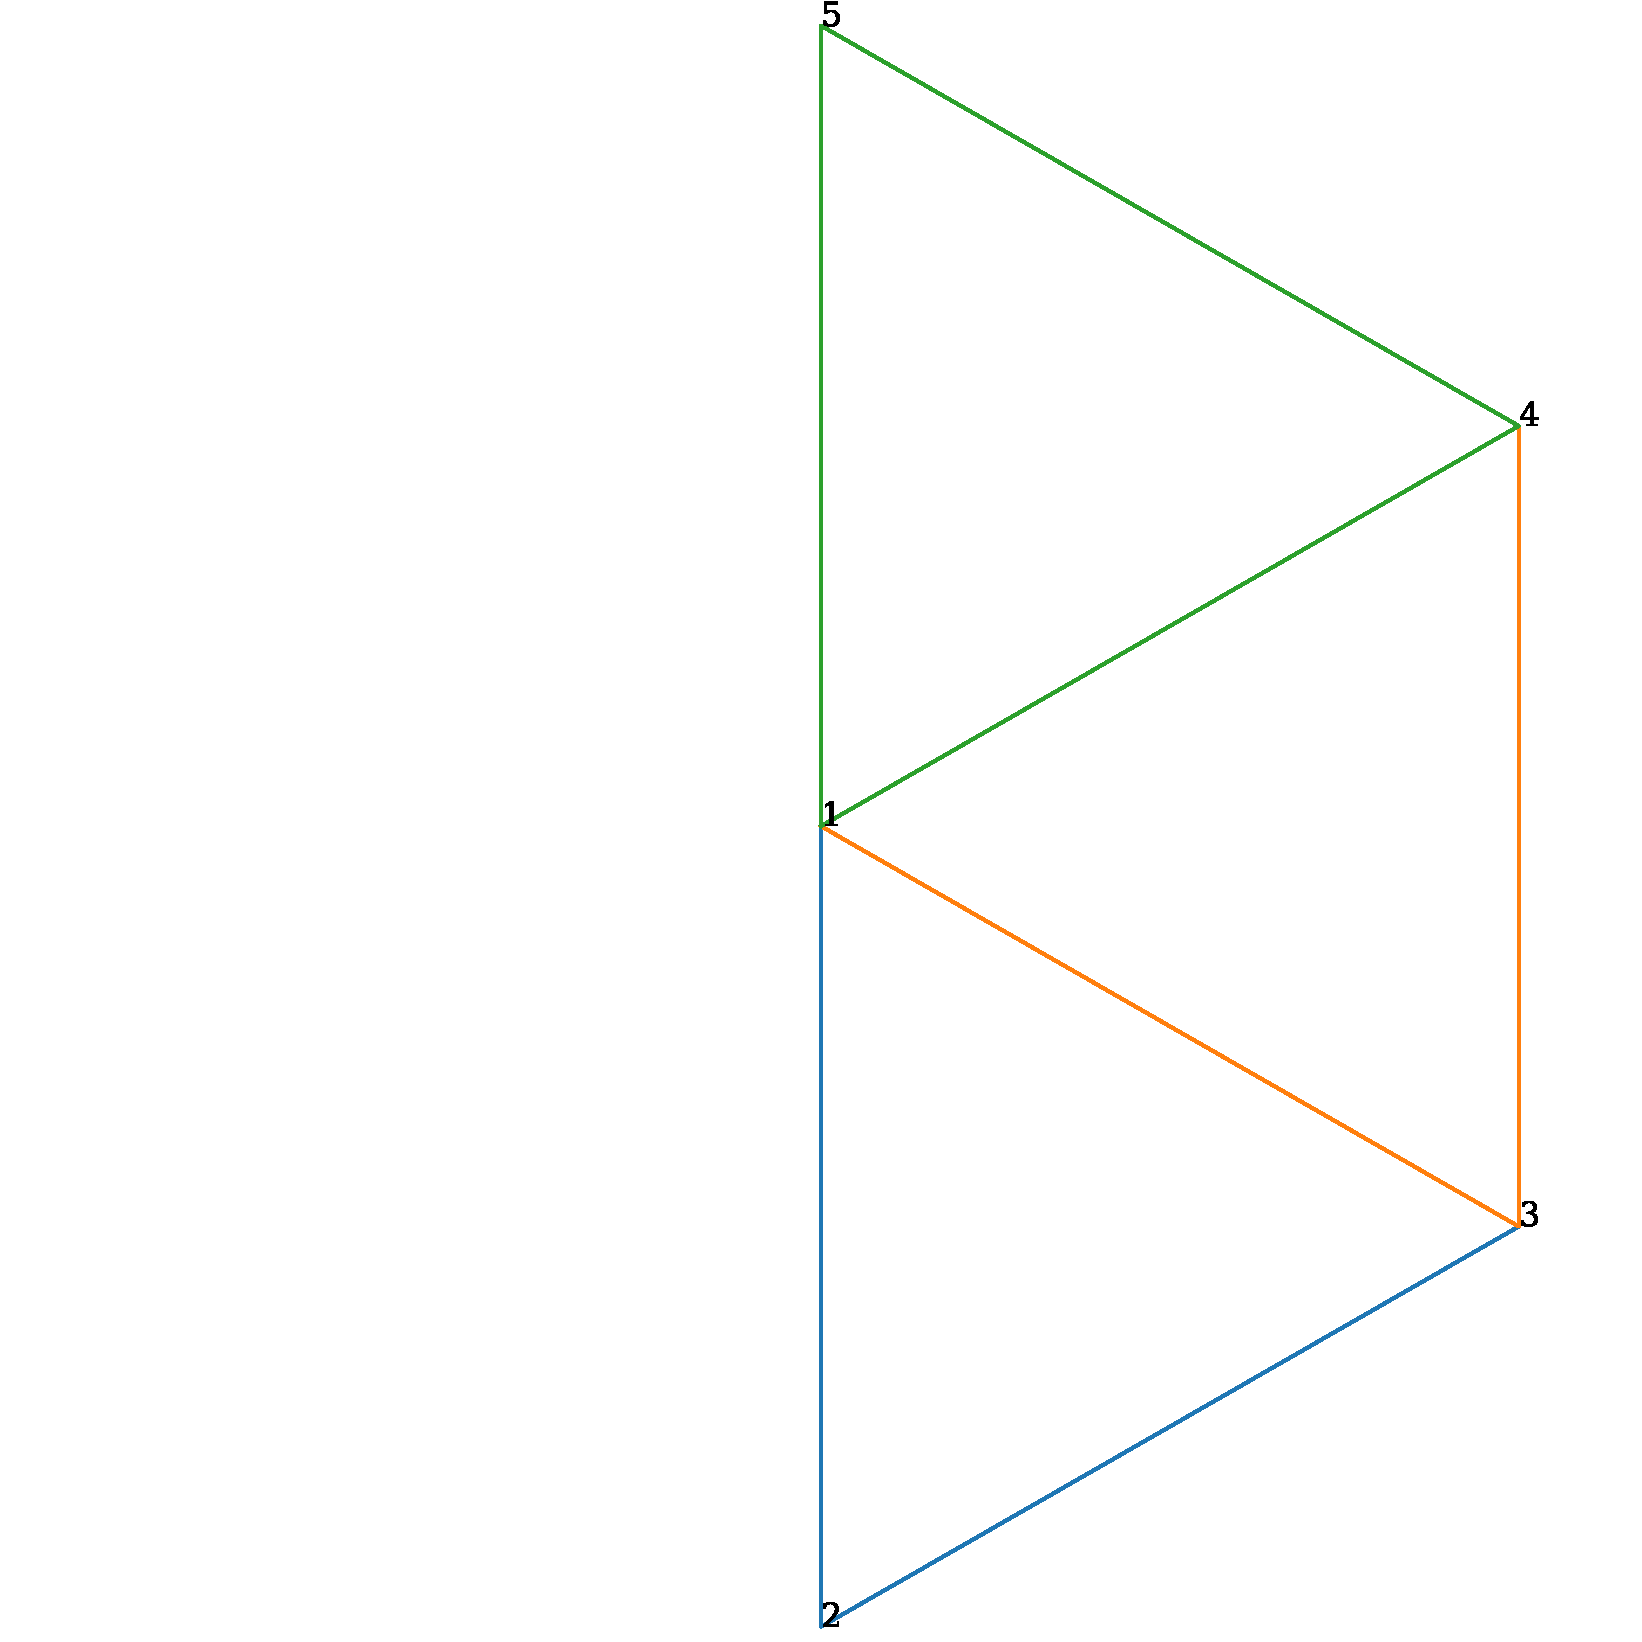
\includegraphics[width=0.5\textwidth]{./mesh_44.pdf}
    \caption{This mesh has three finite elements and five nodes. The nature of
    FEM is that a domain is split into smaller domains which interact with
    each other at the boundaries. The center node will always be designated as
    the first node and is the node where deflection is measured.}
    \label{fig:mesh44}
\end{figure}
since, with the proper boundary conditions, only half the plate is necessary
to run the FEM. There are three finite elements in this figure, each being
a triangle. Each triangle, or (finite) element has three corners, or nodes.
All elements share at least 2 nodes with other elements. This is important since
this connection is what allows the boundary conditions at the edge to propagate
to center. Note that there are currently more nodes (5) than elements (3).
Another ring may be added as in \cref{fig:mesh45}
\begin{figure}[h]
    \centering
    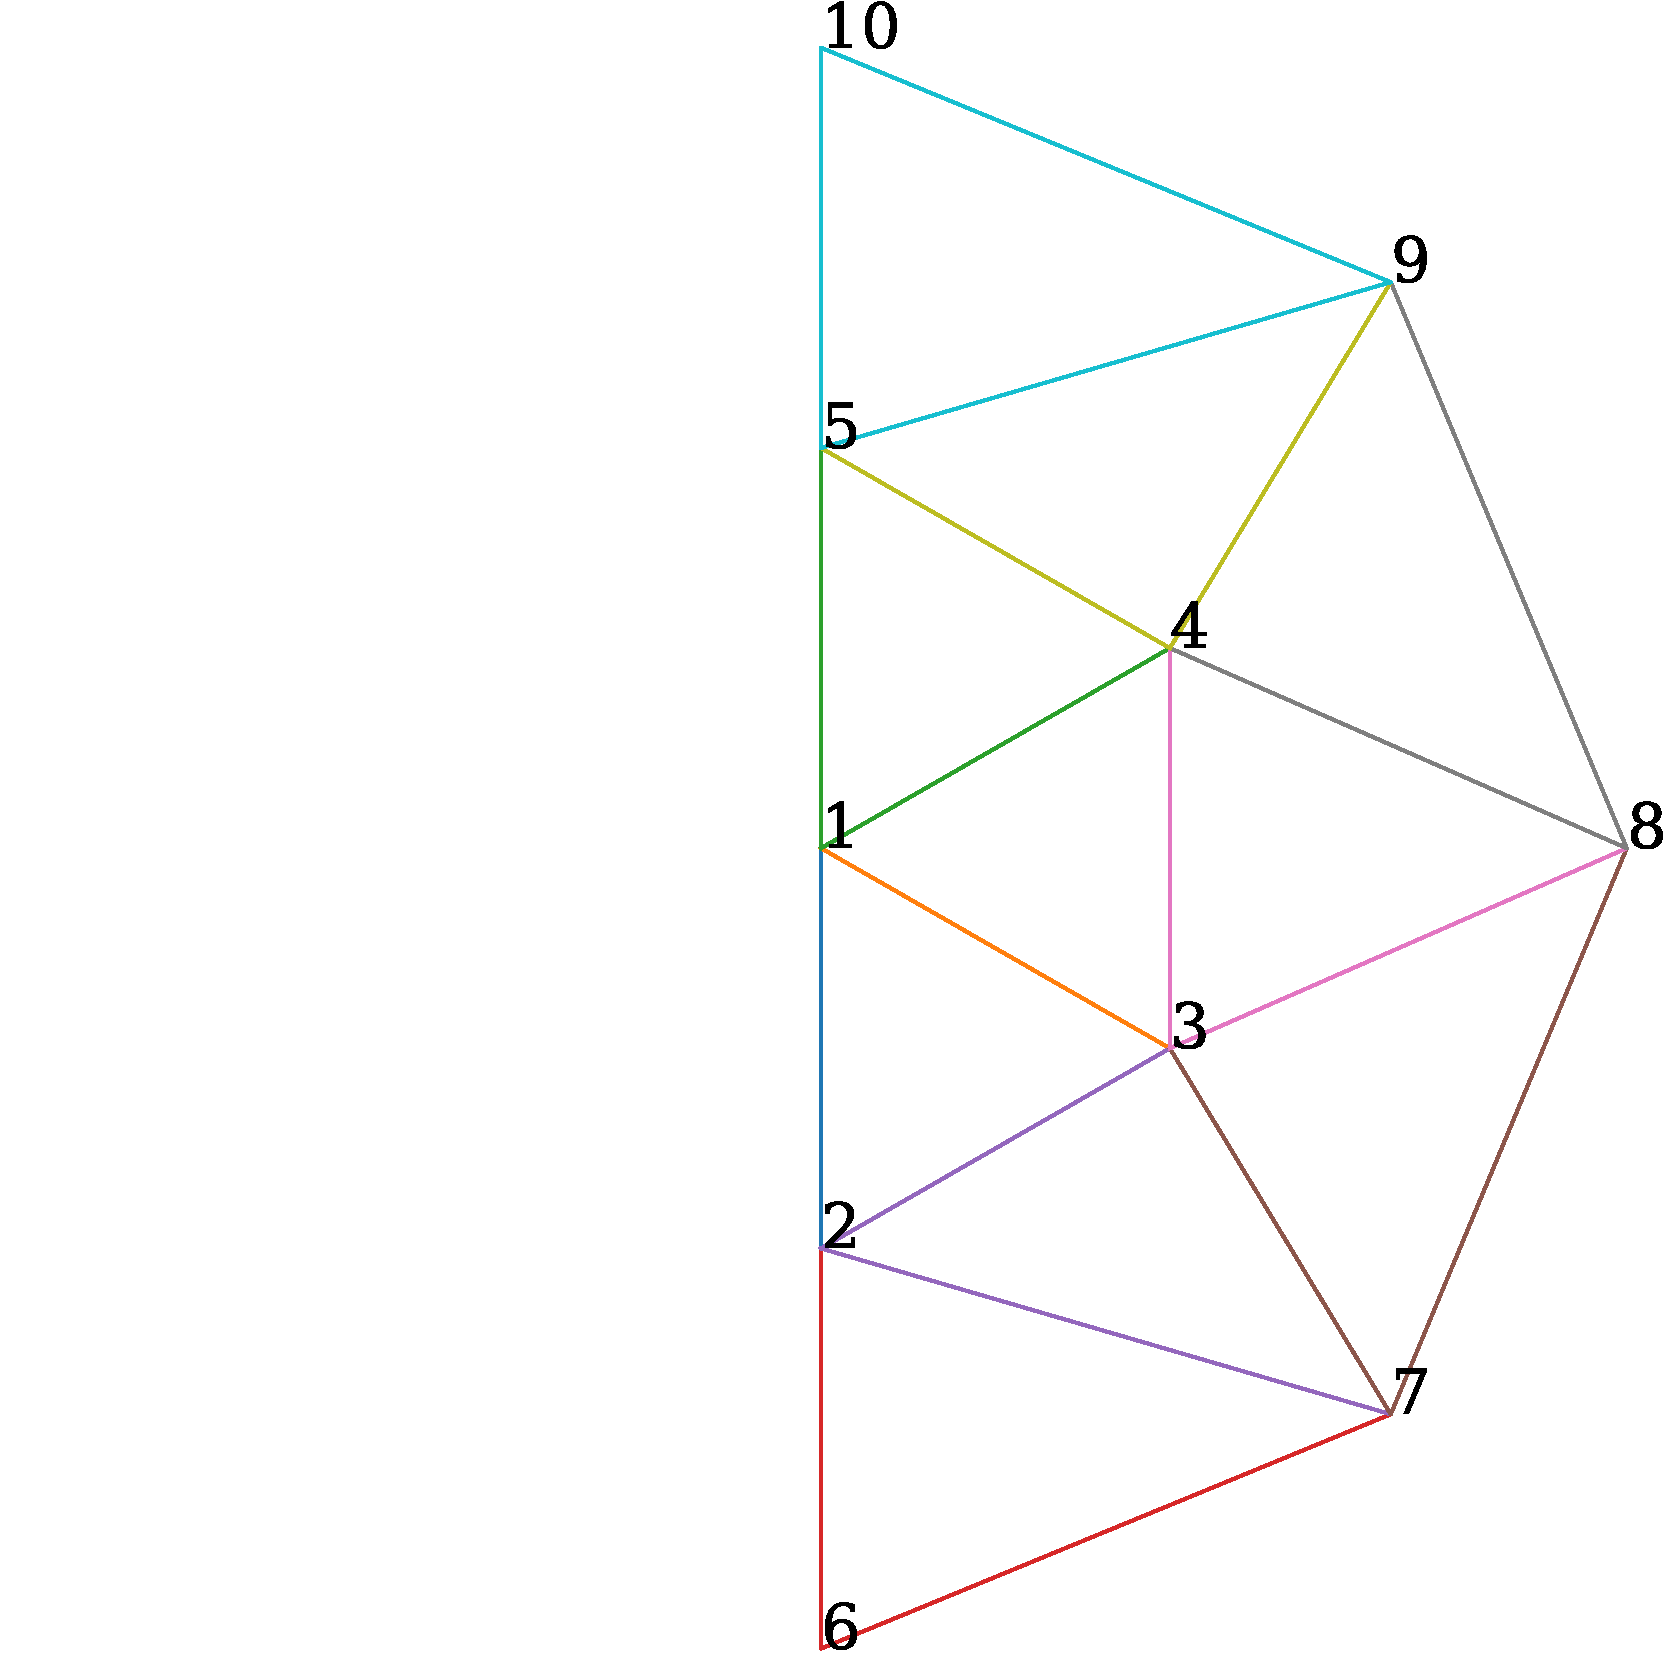
\includegraphics[width=0.5\textwidth]{./mesh_45.pdf}
    \caption{This mesh has ten finite elements and ten nodes. The number of
    elements is related to the number of nodes on a ring as
    $\sum_{i=4}^{5}(2*i-1)$ in this case since there are two rings: the innermost
    ring with 4 nodes and the outermost with 5 nodes. The number of nodes
    will always be lesser than the number of elements past this point.}
    \label{fig:mesh45}
\end{figure}
and now there are an equal number of nodes and elements (10). Note also that while
in \cref{fig:mesh44} the area of each element is clearly equal, this is not the
case for \cref{fig:mesh45}.

A significant amount of time went into programming an algorithm to generate meshes
of arbitrary size, as well as automating the production of these plots. For all
the runs to follow, with the exception of the finite element count scaling run,
a mesh with 898 elements as in \cref{fig:meshm}
\begin{figure}[h]
    \centering
    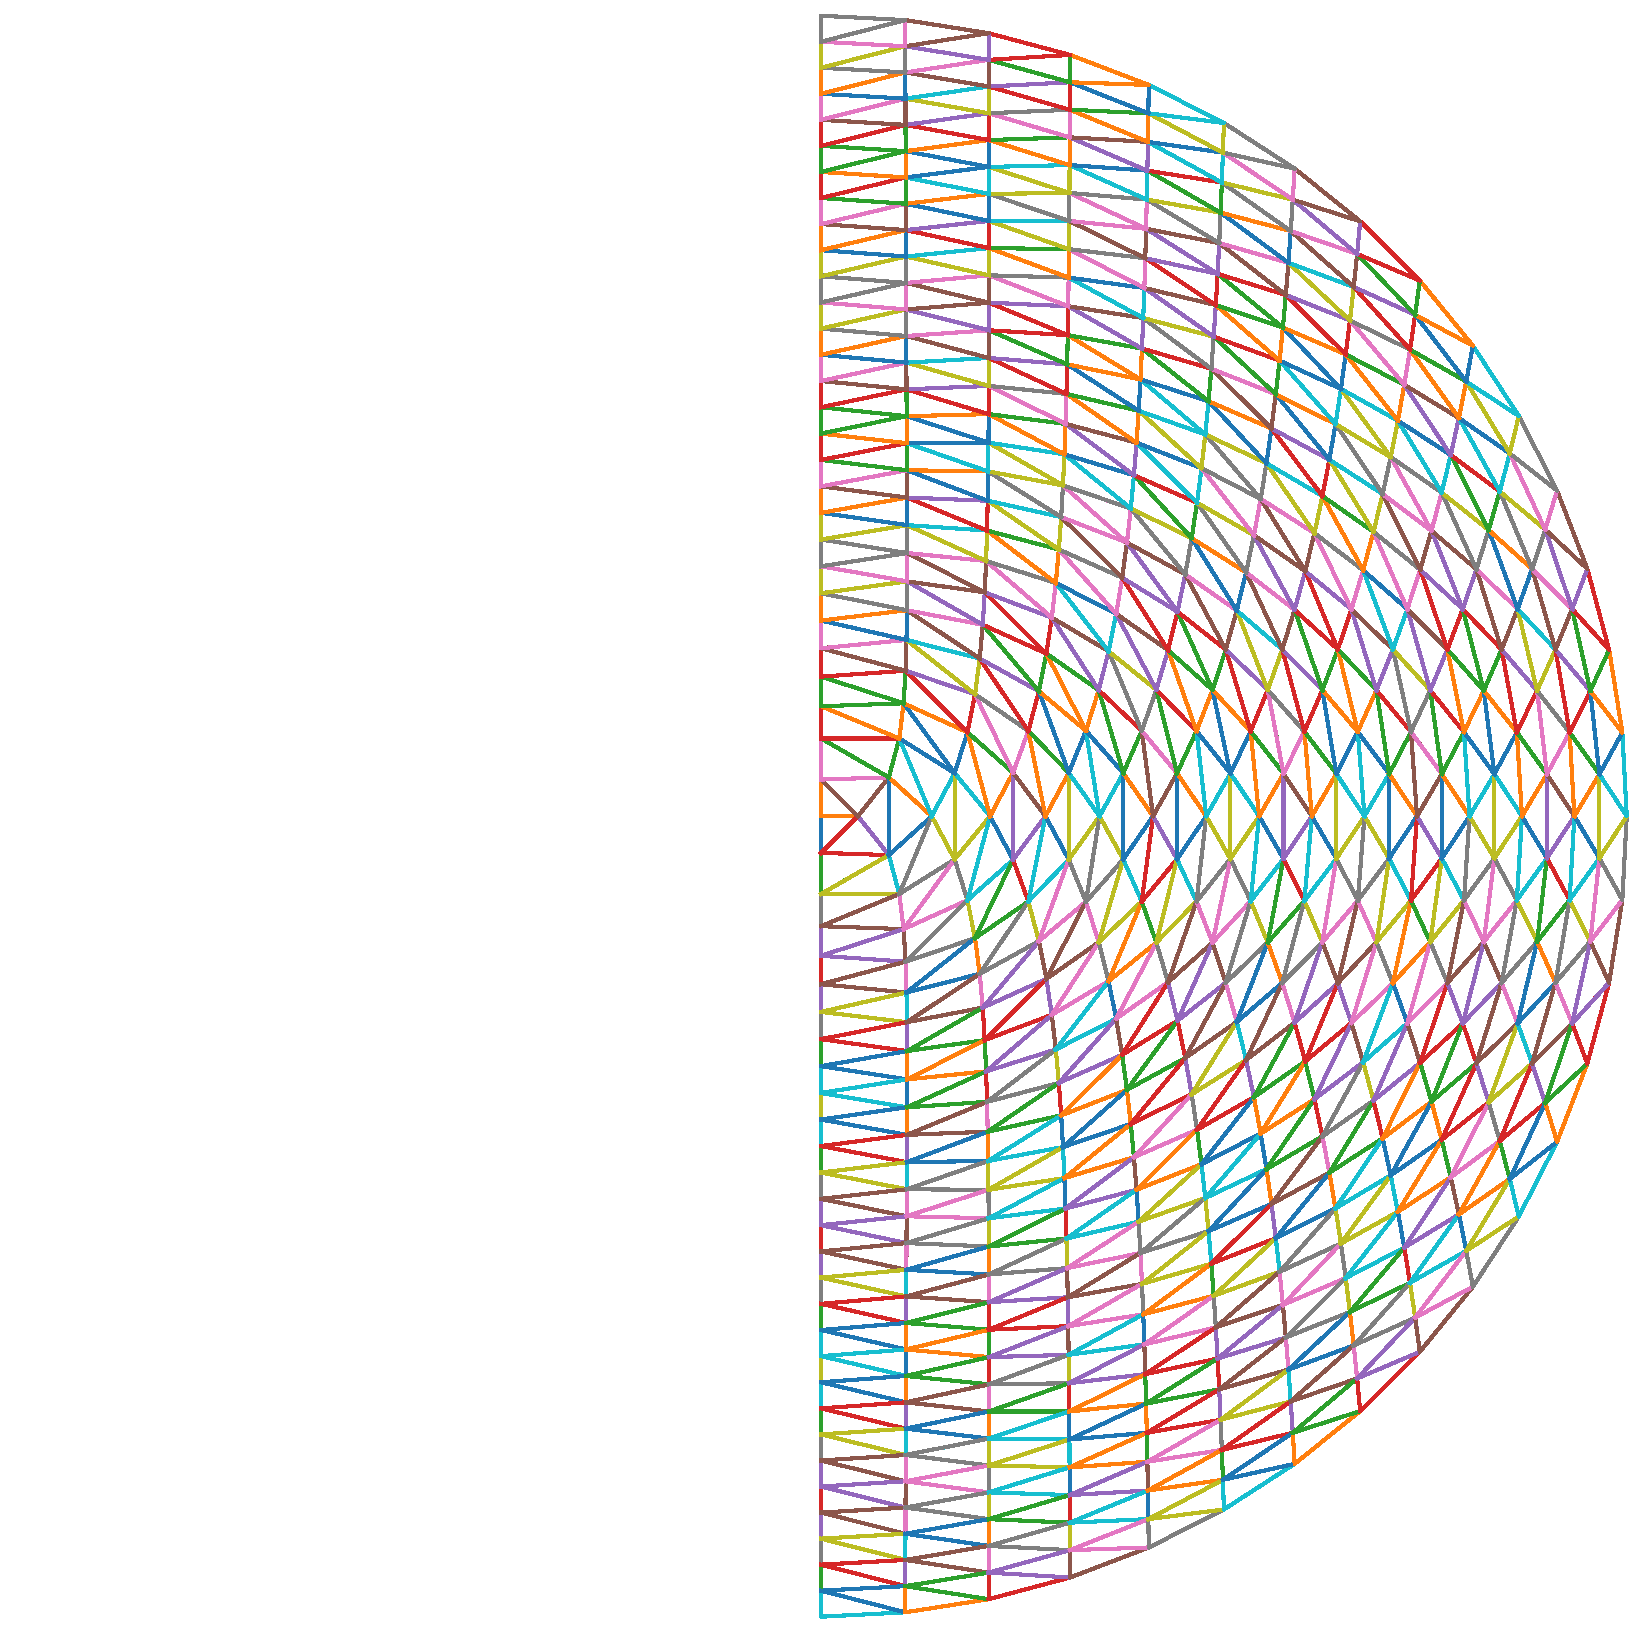
\includegraphics[width=0.5\textwidth]{./mesh_max.pdf}
    \caption{This mesh has 898 finite elements and 494 nodes, and was used for
    the majority of the results in \cref{sec:comp}. The elements near
    center are concerning since they have more area than those near the edge, and
    in general the area appears irregular about center. There is also an open question
    as to whether the general orientation of finite elements is important.}
    \label{fig:meshm}
\end{figure}
was used. While none of the meshes have finite elements with precisely the same
area, which is important since the area determines the amount of pressure a single
finite element feels and therefor affects its relative contribution to the mesh, as
the number of elements scales up the standard deviation goes down: we approach the continuum
limit.

Finally it warrants discussing the expansion of the Fortran code mentioned earlier:
the original code was only capable of handling 170 elements. The code was successfully
modified to handle up to 900 elements for this paper.

\section{Comparison} \label{sec:comp}
For this entire section a set of constant were chosen from \cite{boresi}, problem
13.16. Each graph to follow with keep all but one parameter constant, which will
be noted. Consider \cref{tab:params}
\begin{table}[ht]
    \centering
    \begin{tabular}{ ||c|l|| }
        \hline
        $P$ & $\SI{1.4072}{\newton\milli\meter^{-2}}$ \\
        \hline
        $E$ & $\SI{20394}{\newton\milli\meter^{-2}}$ \\
        \hline
        $a$ & $\SI{250.00}{\milli\meter}$ \\
        \hline
        $h$ & $\SI{25.000}{\milli\meter}$ \\
        \hline
        $\nu$ & 0.29000 \\
        \hline
    \end{tabular}
    \caption{These are the parameters used for all graphs to follow. Each graph
    will treat a parameter as tunable while locking the others: the idea is to
    test a range of values. This will help highlight which variables this FEM
    is more sensitive to relative to the analytic method.}
    \label{tab:params}
\end{table}
where the variables correspond to the pressure, Young's modulus, radius, thickness,
and Poisson's ratio respectively. Unless stated otherwise, the mesh will be as in
\cref{fig:meshm} with 898 elements and 494 nodes.

\Cref{fig:ve}
\begin{figure}[h]
    \centering
    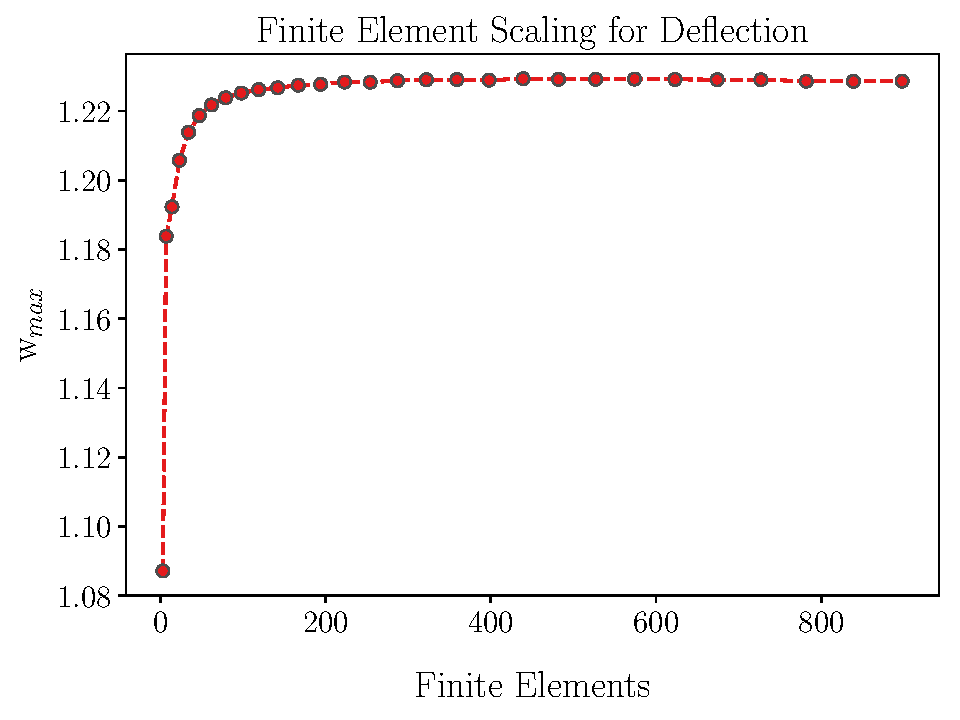
\includegraphics[width=0.5\textwidth]{./ve_scaling.pdf}
    \caption{The density of points is lower on this plot than those to follow because
    of the mesh generation method chosen: not all possible configurations between 4
    and 898 nodes were generated. Parameters used are precisely those used in
    \cref{tab:params}, with the minimum number of elements 3 and the maximum 898.}
    \label{fig:ve}
\end{figure}
considers only the actual deflection as a function of the number of elements used
by the finite element method. There is clearly an asymptotic behavior present, which
seems reasonable since as the number of elements increases their effective area decreases
and we are approaching the continuum limit (that is, moving to the non-finite element
realm) where the actual, exact, solution exists. Consider \cref{tab:ve}
\begin{table}[ht]
    \centering
    \begin{tabular}{ ||c|l|| }
        \hline
        FEM & $\SI{1.2285}{\milli\meter}$ \\
        \hline
        ANA & $\SI{1.2147}{\milli\meter}$ \\
        \hline
    \end{tabular}
    \caption{This is a comparison of the final point in \cref{fig:ve} and the expected
    value from \cref{eqn:def}. The error is within 1.2 percent. Parameters used are
    precisely those used in \cref{tab:params}.}
    \label{tab:ve}
\end{table}
for a comparison to the expected value. It seems that FEM values are reasonably close:
within 1.2 percent. This is encouraging, and so next potential sources of error are
examined by allowing a single parameter to vary, each in turn, while locking the
remaining parameters. Ideally the following plots will either appear random, with a
small variance, or even better flat.

Consider \cref{fig:vpe}
\begin{figure}[h]
    \centering
    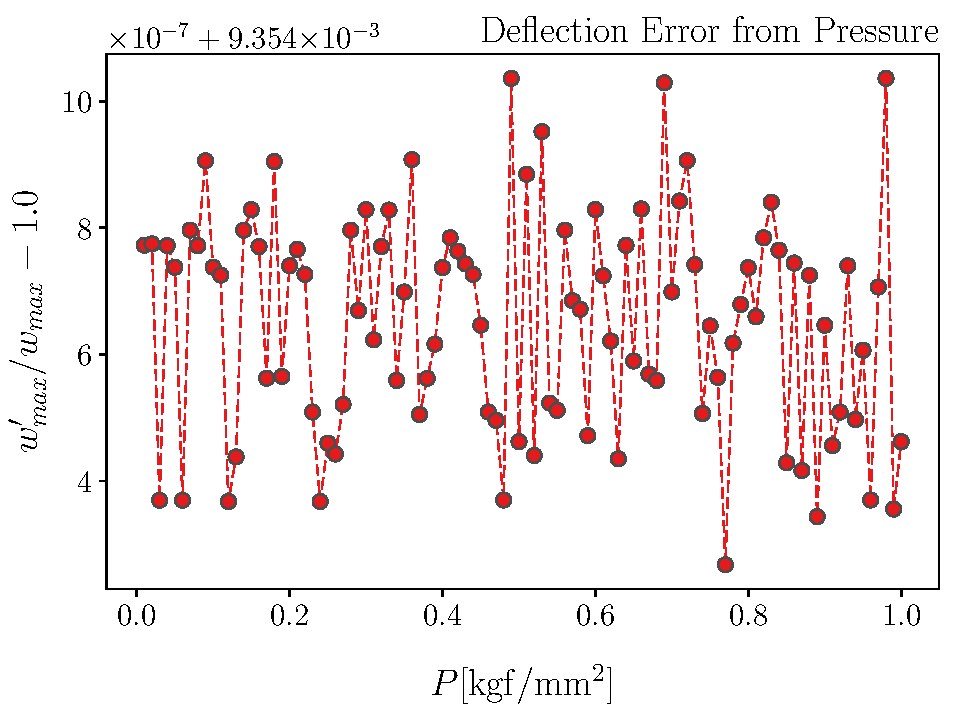
\includegraphics[width=0.5\textwidth]{./yp_scaling_err.pdf}
    \caption{This is another plot of the relative error between the finite
    element method and the analytic method. Note the top left corner: these values
    are all within 0.9 percent error. The parameters used here are as in
    \cref{tab:params}, except that the pressure $P$ varies. The mesh in \cref{fig:meshm}
    was used for all points in all graphs to follow.}
    \label{fig:vpe}
\end{figure}
where pressure is treated as the tunable parameter. Pressure can have a dramatic
effect on the system, being directly related to deflection since it is in a sense
the cause of deflection. It appears however that pressure has little effect on the
error: this looks like noise, and is likely related to the inconsistency of
element area in the generated mesh. Yet taking a second look, note the magnitude
of the error: it is constant, around 0.9 percent. The errors are too large to be
rounding errors. It may be related to the underlying algorithm of the 'Plates'
FEM, specifically the order of the method used to approximate the $\Delta^2$.

Next consider what happens when the ratio between thickness $h$ and $r$, the
radius, becomes the tunable parameter. The expectation is that as this ratio
approaches $1.0$, the error will increase. Unfortunately both the analytic
method and finite element method are derived from the same principles and the
error noted here is relative error between the two: it should be thought of as
a measure of the FEM method as a replacement of the analytic method, not a
measure of how correct either method in the thick plate regime.
\Cref{fig:tre}
\begin{figure}[h]
    \centering
    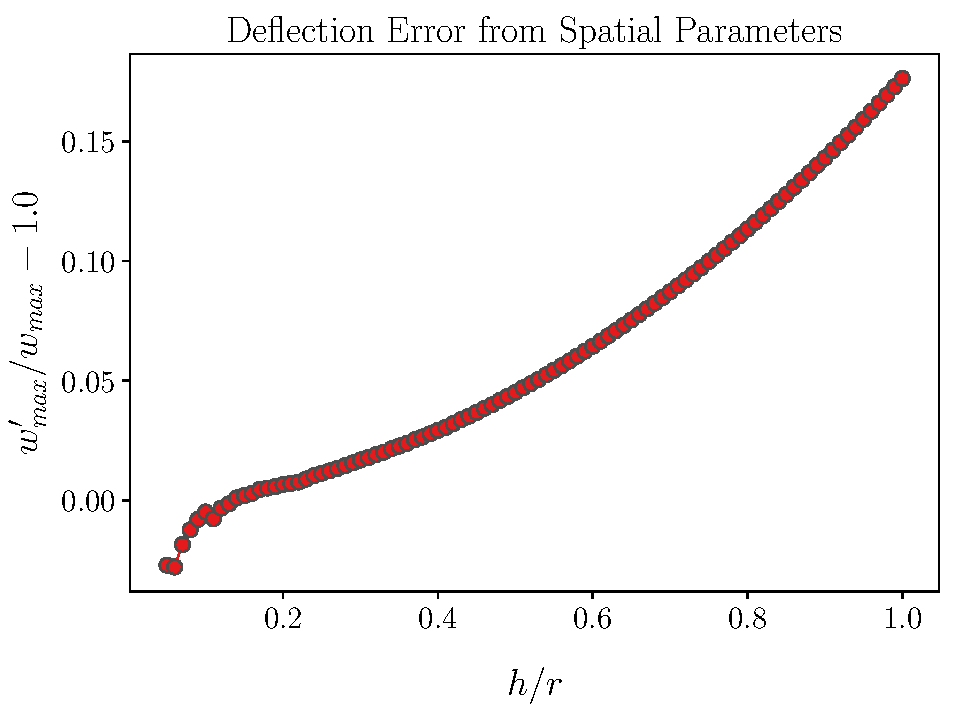
\includegraphics[width=0.5\textwidth]{./tr_scaling_err.pdf}
    \caption{}
    \label{fig:tre}
\end{figure}
shows that the two methods diverge. This divergence is in favor of the FEM method.
Experiments have shown that as thickness increases, the calculated deflection is
much less than the measured and in fact a prefactor
\begin{equation} \label{eqn:pre}
    C = 1 + 5.72\left(\frac{h}{a}\right)^2
\end{equation}
is necessary, with $a$ as the radius to match \cref{eqn:def}.

Now a look at the material parameters, Young's modulus and Poisson's ratio, remains.
Considering \cref{eqn:def}, Young's modulus $E$ is of the same order as the pressure $P$.
This suggests any errors should also be on the same order, specifically varying $E$
isn't expected to cause the two methods to diverge. \Cref{fig:vre}
\begin{figure}[h]
    \centering
    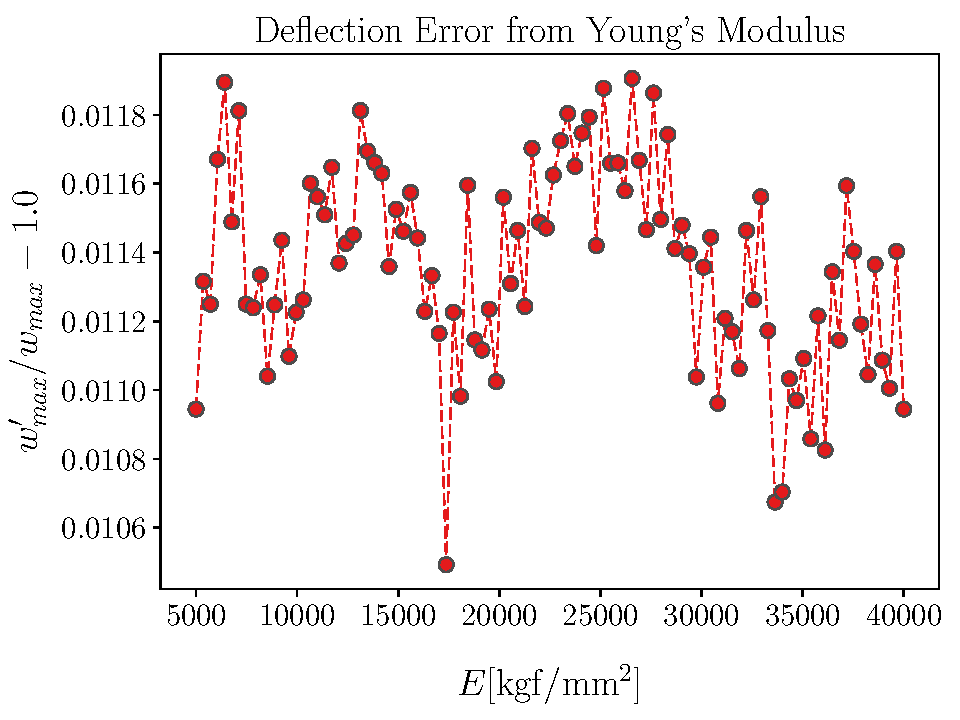
\includegraphics[width=0.5\textwidth]{./ym_scaling_err.pdf}
    \caption{}
    \label{fig:vre}
\end{figure}
supports this expectation with what seems a constant error, however the magnitude
is within 1.2 percent, slightly larger than the 0.9 percent found with pressure.

\section{Discussion} \label{sec:disc}

%% The Appendices part is started with the command \appendix;
%% appendix sections are then done as normal sections
%% \appendix

%% \section{}
%% \label{}

\bibliographystyle{elsarticle-num} 
\bibliography{refs.bib}

\end{document}
\endinput
%%
%% End of file `elsarticle-template-num.tex'.
